\documentclass[11pt]{article}
\usepackage[utf8]{inputenc}	% Para caracteres en español
\usepackage{amsmath,amsthm,amsfonts,amssymb,amscd}
\usepackage{multirow,booktabs}
\usepackage[table]{xcolor}
\usepackage{fullpage}
\usepackage{lastpage}
\usepackage{enumitem}
\usepackage{fancyhdr}
\usepackage{mathrsfs}
\usepackage{wrapfig}
\usepackage{setspace}
\usepackage{calc}
\usepackage{multicol}
\usepackage{cancel}
\usepackage{float}
\usepackage{physics}
\usepackage[retainorgcmds]{IEEEtrantools}
\usepackage[margin=1cm]{geometry}
\usepackage{amsmath}
\newlength{\tabcont}
\setlength{\headheight}{14pt}
\setlength{\parindent}{0.0in}
\setlength{\parskip}{0.05in}
\usepackage{empheq}
\usepackage{framed}
\usepackage[most]{tcolorbox}
\usepackage{xcolor}
\usepackage[version=3]{mhchem}
\usepackage[english]{babel}
\usepackage[utf8]{inputenc}
\usepackage{graphicx}
\usepackage[colorinlistoftodos]{todonotes}
\usepackage{mdframed}

\colorlet{shadecolor}{orange!15}
\parindent 0in
\parskip 12pt
\geometry{margin=1in, headsep=0.25in}
\theoremstyle{definition}
\newtheorem{defn}{Definition}
\newtheorem{reg}{Rule}
\newtheorem{exer}{Exercise}
\newtheorem{note}{Note}
\begin{document}
\setcounter{section}{2}
%\setcounter{subsection}{}
\title{Problem Set 7}

%==============================================================
%\thispagestyle{empty}
\pagestyle{fancy}
\fancyhf{}
\rhead{Physics 180}
\chead{Problem Set 7}
\lhead{Olyn D. Desabelle}
\rfoot{Page \thepage}

\begin{center}
{\LARGE \bf Problem Set 7}\\
%{\large Physics 180}\\
%Olyn D. Desabelle
\end{center}

\begin{figure}[H]
    \centering
    \includegraphics[scale = 0.5]{5.1.png}
\end{figure}
\begin{figure}[H]
    \centering
    \includegraphics[scale = 0.5]{fig 5.5.png}
\end{figure}

For the given s-channel, the processes can have different sequences on which they happened, as all we know is that there are incoming $a$ and $b$ and outgoing $c$ and $d$. For one, an incoming $a$ splits into an outgoing $c$ and $X$, and this $X$ then interacts with an incoming $b$ to produce $d$. In another, $c$, $d$, and $X$ are produced first, then incoming $a$ and $b$ interact with $X$ to disappear. These time orderings may be represented as:

\begin{figure}[H]
    \centering
    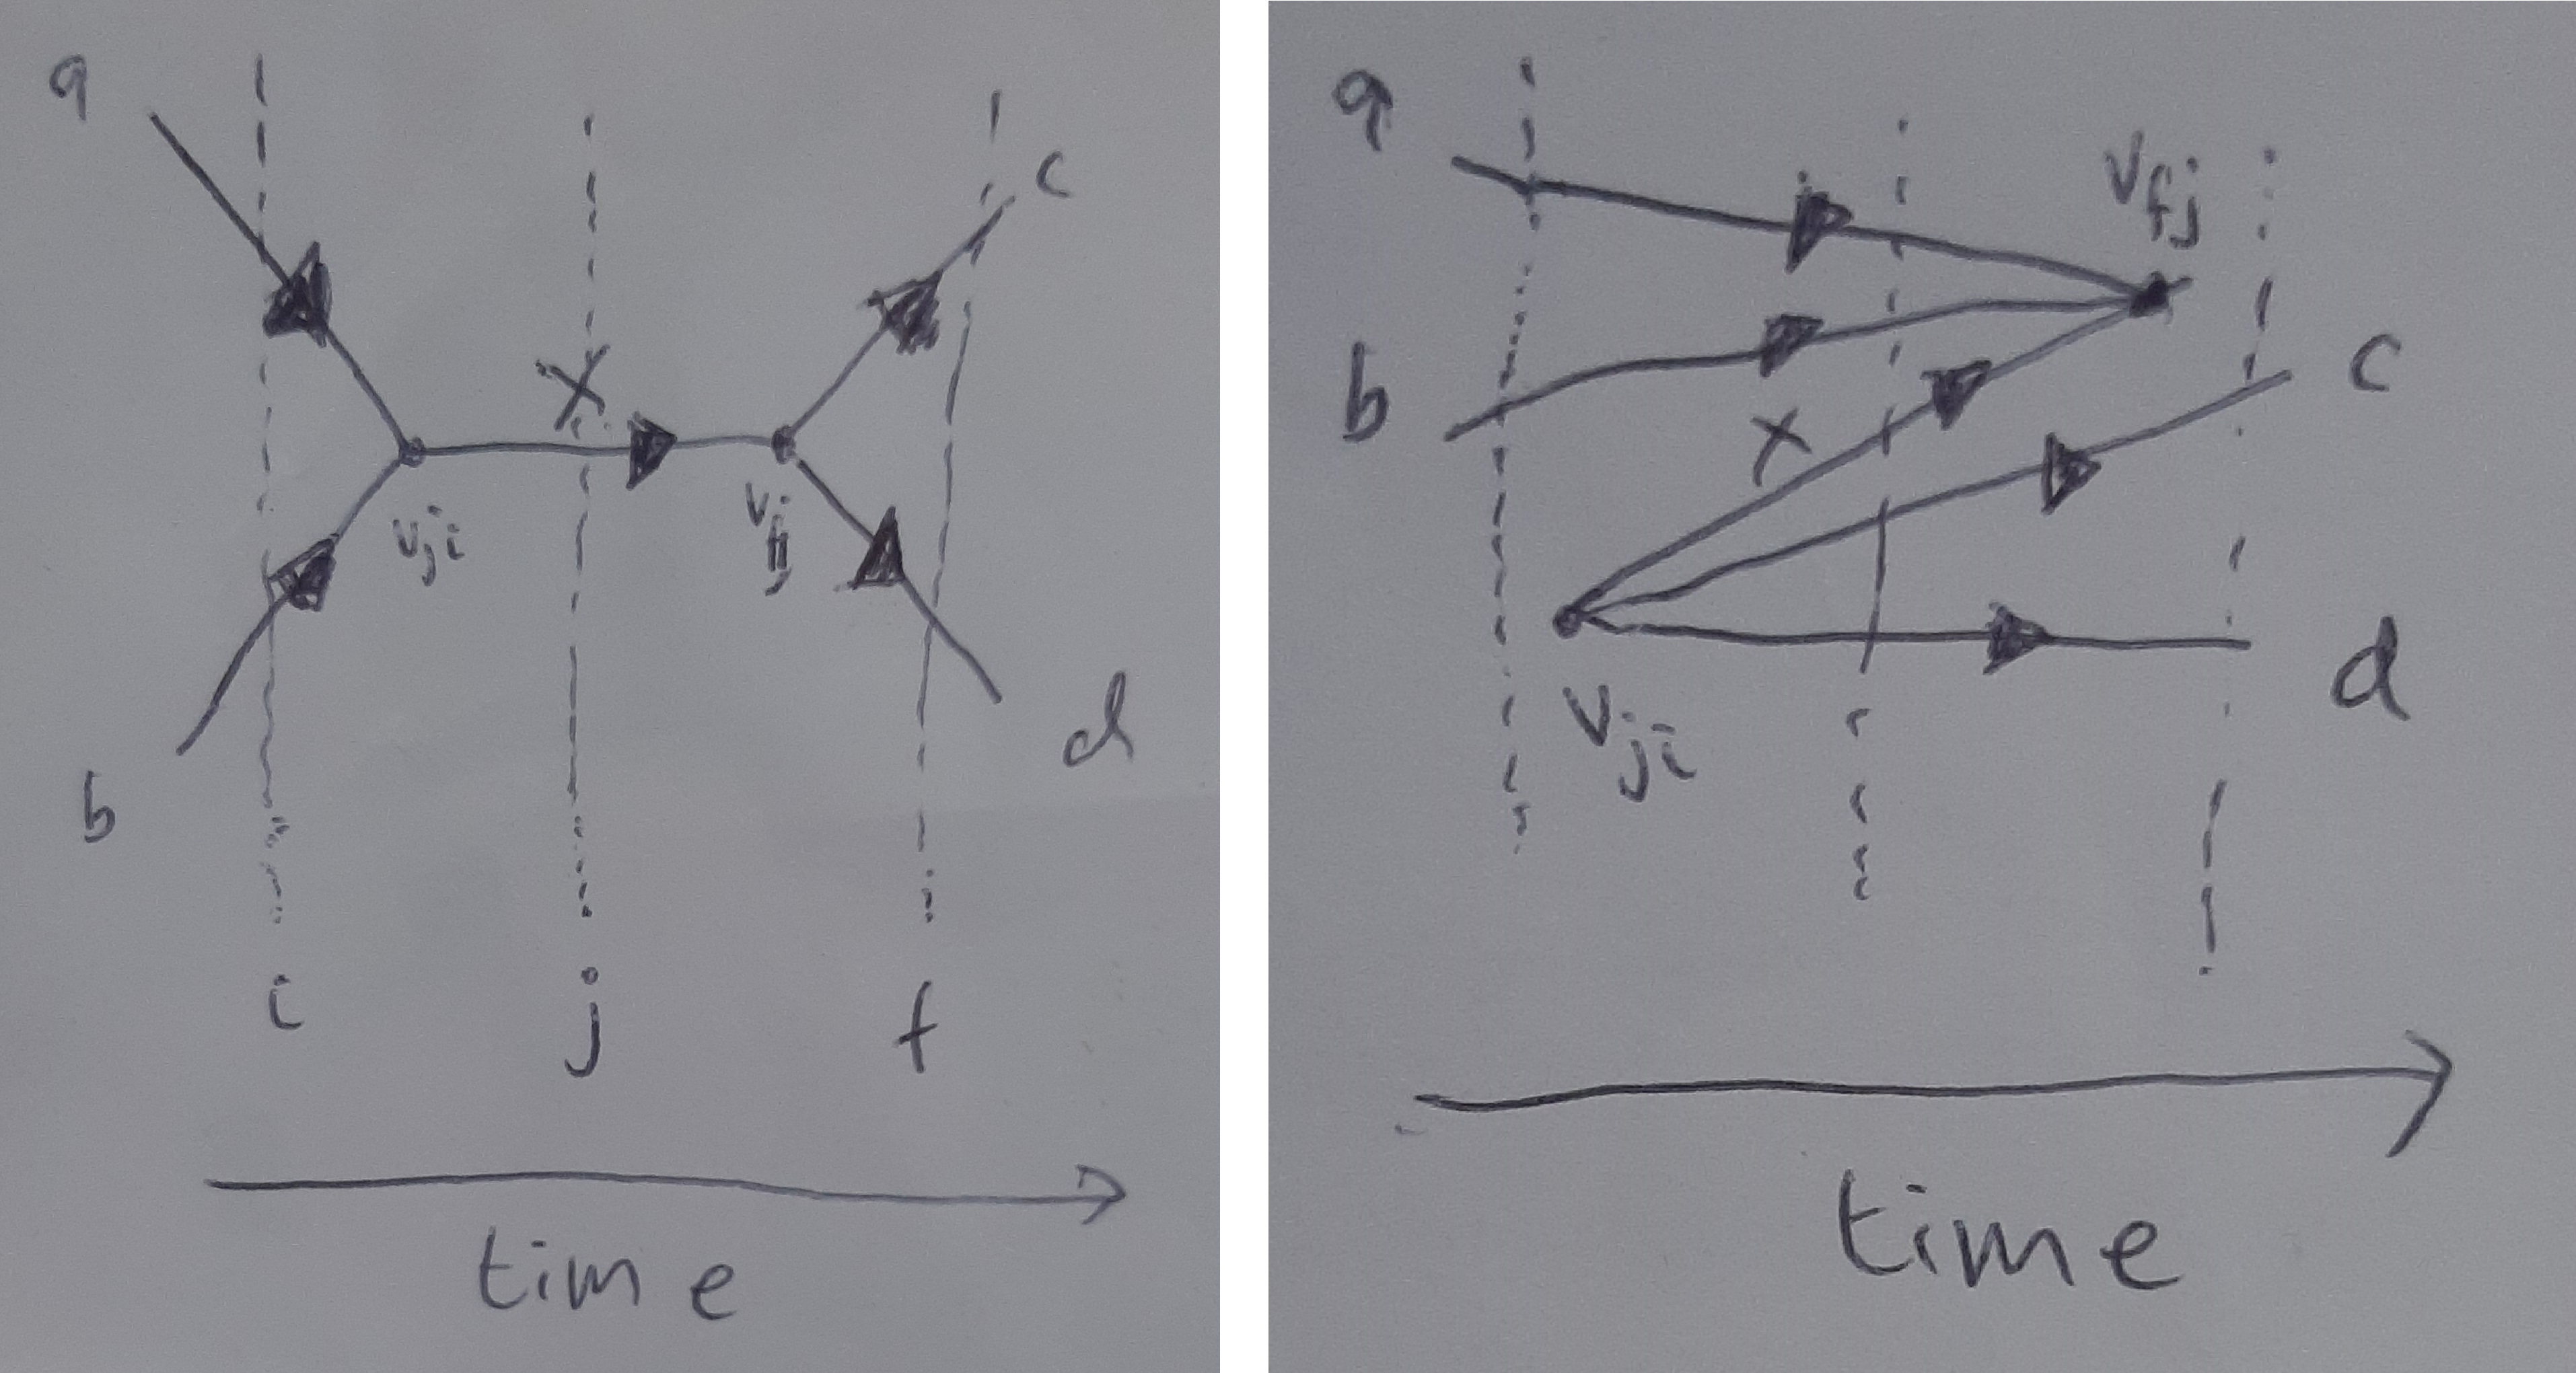
\includegraphics[scale = 0.1]{s-channels.png}
\end{figure}

For the first time ordering, we may obtain the transition matrix element $T_{fi}^{ab}$ as given by Equation 5.1 and by noting the different regions ($c$ and $d$ in the $f$ region, $X$ in the $j$ region, and $a$ and $b$ in the $i$ region):

\begin{align}
    T_{fi}^{ab} &= 
    \frac{\bra{f}V\ket{j}\bra{j}V\ket{i}}
    {E_i-E_j}\\
    T_{fi}^{ab} &= 
    \frac{\bra{c+d}V\ket{X}\bra{X}V\ket{a+b}}
    {(E_a+E_b)-E_X}\\
\end{align}

The non-invariant matrix elements $ \bra{f}V\ket{j}$ and $ \bra{j}V\ket{i}$ are given by:

\begin{align}
    \bra{f}V\ket{j} = \bra{c+d}V\ket{X} &=
    \mathcal{M}_{fj} \prod_k (2E_k)^{-1/2}\\
    \bra{j}V\ket{i} = \bra{X}V\ket{a+b} &=
    \mathcal{M}_{ji} \prod_k (2E_k)^{-1/2}\\
\end{align}

we can also rewrite the matrix as the coupling constants:

\begin{align}
    \mathcal{M}_{fj}\mathcal{M}_{ji} = g_ag_b= g^2
\end{align}

thus we have:

\begin{align}
    T_{fi}^{ab} &= 
    \frac{1}{2E_X \cdot 2(2E_aE_bE_cE_d)^{1/2}}
    \frac{g^2}
    {(E_a+E_b)-E_X}\\
\end{align}

we can get the overall Lorentz-invariant matrix in the form of:

\begin{align}
    \mathcal{M}_{fi}^{ab} &= 2(2E_aE_bE_cE_d)^{1/2} T_{fi}^{ab}\\
    \mathcal{M}_{fi}^{ab} &= \frac{1}{2E_X} \frac{g^2}{(E_a+E_b)-E_X}
\end{align}

we repeat the same steps for the second time ordering:

\begin{align}
    T_{fi}^{cd} &= 
    \frac{\bra{f}V\ket{j}\bra{j}V\ket{i}}
    {E_i-E_j}\\
    T_{fi}^{cd} &= 
    \frac{\bra{c+d+X}V\ket{0}\bra{0}V\ket{a+b+X}}
    {(E_a+E_b)-(E_a+E_b+E_c + E_d + E_X)}\\
\end{align}

with $E_c+E_d = E_a+E_b$, we have:

\begin{align}
    T_{fi}^{cd} &= 
    \frac{1}{2E_X \cdot 2(2E_aE_bE_cE_d)^{1/2}}
    \frac{g^2}
    {-E_a - E_b - E_X}\\
\end{align}

we proceed with obtaining the matrix element:

\begin{align}
    \mathcal{M}_{fi}^{cd} &= 2(2E_aE_bE_cE_d)^{1/2} T_{fi}^{cd}\\
    \mathcal{M}_{fi}^{cd} &= -\frac{1}{2E_X} \frac{g^2}{(E_a+E_b)+E_X}
\end{align}

to get the combined Lorentz-invariant matrix element of both time orderings, we get their sum:

\begin{align}
    \mathcal{M} &=
    \mathcal{M}_{fi}^{ab}+\mathcal{M}_{fi}^{cd}\\
    \mathcal{M} &= \left[\frac{1}{2E_X} \frac{g^2}{(E_a+E_b)-E_X}\right] + \left[-\frac{1}{2E_X} \frac{g^2}{(E_a+E_b)+E_X}\right]\\
    \mathcal{M} &= \frac{g^2}{2E_X} \left[ \frac{1}{(E_a+E_b)-E_X} - \frac{1}{(E_a+E_b)+E_X} \right]\\
    \mathcal{M} &= \frac{g^2}{2E_X} \left[ \frac{2E_X}{(E_a+E_b)^2 - E_X^2} \right]\\
\end{align}

we can rewrite $E_X^2$ as:

\begin{align}
    E_X^2 &= \mathbf{p}_X^2 + m_X^2\\
    E_X^2 &= (\mathbf{p}_a + \mathbf{p}_b)^2 + m_X^2
\end{align}

thus the matrix element becomes:

\begin{align}
    \mathcal{M} &= \frac{g^2}{(E_a+E_b)^2 - (\mathbf{p}_a + \mathbf{p}_b)^2 - m_X^2}\\
    \mathcal{M} &= \frac{g^2}{ (p_a + p_b)^2 - m_X^2} 
\end{align}

rewriting this in terms of the Mandelstam $s$ variable $q=(p_a + p_b)^2$, we get:

\begin{align}
    \mathcal{M} &= \frac{g^2}{ q^2 - m_X^2}
\end{align}

\begin{mdframed}
    This form recovers the $\frac{1}{q^2 - m_X^2}$ propagator.
\end{mdframed}
%we then note that we can switch up the order of differentiation:

%\begin{align*}
%    \gamma^{\nu}\gamma^{\mu} \partial_{\nu}\partial_{\mu} = \gamma^{\mu}\gamma^{\nu} \partial_{\mu}\partial_{\nu}\\
%    2\gamma^{\nu}\gamma^{\mu} \partial_{\nu}\partial_{\mu} = \gamma^{\mu}\gamma^{\nu} \partial_{\mu}\partial_{\nu} +  \gamma^{\nu}\gamma^{\mu} \partial_{\nu}\partial_{\mu}\\
%\end{align*}


%==============================================================
\newpage
%==============================================================

\begin{figure}[H]
    \centering
    \includegraphics[scale = 0.55]{5.3.png}
\end{figure}

In the case of $e^{+}e^{-}\to\gamma\gamma$, two identical particles are produced. Hence, we use either t-channel or u-channel diagrams. The t-channel diagram generally looks like:

\begin{figure}[H]
    \centering
    \includegraphics[scale = 0.1]{general t-channel.jpg}
\end{figure}

we can place the particles given into the above general configuration:

\begin{figure}[H]
    \centering
    \includegraphics[scale = 0.1]{t-channel with particles.jpg}
\end{figure}

reconfiguring this so that particle arrows go with the time arrow, antiparticle arrows go against the time arrow, each vertex has one $\gamma$ photon as allowed in vertex rules, and having the fermion propagator as the virtual particle, we have:

\begin{figure}[H]
    \centering
    \includegraphics[scale = 0.1]{final t-channel.jpg}
\end{figure}

we note the following contributions to the matrix element $-i\mathcal{M}_t$:

\begin{align*}
    \text{initial state particle }(e^{-}) \; &: \; u(p)\\
    \text{initial state antiparticle }(e^{+}) \; &: \; \bar{v}(p)\\
    \text{final state photons }(\gamma) \; &: \; \varepsilon^{*}_{\mu}(p)\\
    \text{fermion propagator }(q) \; &: \; -\frac{i(\gamma^{\mu} q_{\mu} + m)}{q^2-m^2}\\
    \text{interaction vertex factor } \; &: \; ie\gamma^{\mu}\\
\end{align*}

the product of the contributions from the initial state electron at the 1 position and the final state photon at position 3 along with the corresponding interaction vertex factor is given by:

\begin{align}
    \varepsilon^{*}_{\mu}(p)ie\gamma^{\mu}u(p)\\
    \varepsilon^{*}_{\mu}(p_3)ie\gamma^{\mu}u(p_1)\\
\end{align}

the product of the contributions from the initial state positron at the 2 position and the final state photon at position 4 along with the corresponding interaction vertex factor is given by:

\begin{align}
    \varepsilon^{*}_{\nu}(p)ie\gamma^{\nu}\bar{v}(p)\\
    \varepsilon^{*}_{\nu}(p_4)ie\gamma^{\nu}\bar{v}(p_2)\\
\end{align}

lastly, we have the fermion propagator in the middle:

\begin{align}
    -\frac{i(\gamma^{\mu} q_{\mu} + m)}{q^2-m^2}\\
\end{align}

thus for the matrix element of the t-channel diagram, rearranging the terms such that the initial state electron and positron terms are nearer to the fermion propagator, we have:

\begin{align}
    -i\mathcal{M}_t = 
    \left[
        \varepsilon^{*}_{\mu}(p_3)ie\gamma^{\mu}u(p_1)
    \right]
    \left[
        -\frac{i(\gamma^{\mu} q_{\mu} + m)}{q^2-m^2}
    \right]
    \left[
        \bar{v}(p_2)ie\gamma^{\nu}\varepsilon^{*}_{\nu}(p_4)
    \right]
\end{align}

\begin{equation}
\boxed{
    \mathcal{M}_t = 
    \left[
        \varepsilon^{*}_{\mu}(p_3)e\gamma^{\mu}u(p_1)
    \right]
    \left[
        -\frac{(\gamma^{\mu} q_{\mu} + m)}{q^2-m^2}
    \right]
    \left[
        \bar{v}(p_2)e\gamma^{\nu}\varepsilon^{*}_{\nu}(p_4)
    \right]
}
\end{equation}

for the u-channel diagram, we have the general configuration:

\begin{figure}[H]
    \centering
    \includegraphics[scale = 0.1]{general u-channel.jpg}
\end{figure}

particles inserted along with the proper corrections, we have:

\begin{figure}[H]
    \centering
    \includegraphics[scale = 0.1]{final u-channel.jpg}
\end{figure}

we notice from the general diagram that particle 4 and 3 just switched, and thus for its matrix elements $\mathcal{M}_u$ we can interchange the terms referring to those particles from the earlier $\mathcal{M}_t$:

\begin{equation}
    \boxed{
        \mathcal{M}_u = 
        \left[
            \varepsilon^{*}_{\mu}(p_4)e\gamma^{\mu}u(p_1)
        \right]
        \left[
            -\frac{(\gamma^{\mu} q_{\mu} + m)}{q^2-m^2}
        \right]
        \left[
            \bar{v}(p_2)e\gamma^{\nu}\varepsilon^{*}_{\nu}(p_3)
        \right]
    }
    \end{equation}
%we note that in our earlier solution evaluating $\gamma^{0}\gamma^{0}\gamma^{0}$, we found that $\gamma^{0}\gamma^{0} = \begin{pmatrix}1&0&0&0\\ 0&1&0&0\\ 0&0&1&0\\ 0&0&0&1\end{pmatrix} = I$. Thus we can rewrite the LHS of the equation as:

%\begin{align*}
%    -\gamma^{k} = -I\gamma^{k}\\
%    -\gamma^{k} = -\gamma^{0}\gamma^{0}\gamma^{k}
%\end{align*}

%we can rewrite the RHS of the equation as:

%\begin{align*}
%    \gamma^{0}\gamma^{k}\gamma^{0} = 
%\end{align*}
%==================================
\end{document}